%%
% Copyright (c) 2017 - 2020, Pascal Wagler;
% Copyright (c) 2014 - 2020, John MacFarlane
%
% All rights reserved.
%
% Redistribution and use in source and binary forms, with or without
% modification, are permitted provided that the following conditions
% are met:
%
% - Redistributions of source code must retain the above copyright
% notice, this list of conditions and the following disclaimer.
%
% - Redistributions in binary form must reproduce the above copyright
% notice, this list of conditions and the following disclaimer in the
% documentation and/or other materials provided with the distribution.
%
% - Neither the name of John MacFarlane nor the names of other
% contributors may be used to endorse or promote products derived
% from this software without specific prior written permission.
%
% THIS SOFTWARE IS PROVIDED BY THE COPYRIGHT HOLDERS AND CONTRIBUTORS
% "AS IS" AND ANY EXPRESS OR IMPLIED WARRANTIES, INCLUDING, BUT NOT
% LIMITED TO, THE IMPLIED WARRANTIES OF MERCHANTABILITY AND FITNESS
% FOR A PARTICULAR PURPOSE ARE DISCLAIMED. IN NO EVENT SHALL THE
% COPYRIGHT OWNER OR CONTRIBUTORS BE LIABLE FOR ANY DIRECT, INDIRECT,
% INCIDENTAL, SPECIAL, EXEMPLARY, OR CONSEQUENTIAL DAMAGES (INCLUDING,
% BUT NOT LIMITED TO, PROCUREMENT OF SUBSTITUTE GOODS OR SERVICES;
% LOSS OF USE, DATA, OR PROFITS; OR BUSINESS INTERRUPTION) HOWEVER
% CAUSED AND ON ANY THEORY OF LIABILITY, WHETHER IN CONTRACT, STRICT
% LIABILITY, OR TORT (INCLUDING NEGLIGENCE OR OTHERWISE) ARISING IN
% ANY WAY OUT OF THE USE OF THIS SOFTWARE, EVEN IF ADVISED OF THE
% POSSIBILITY OF SUCH DAMAGE.
%%

%%
% This is the Eisvogel pandoc LaTeX template.
%
% For usage information and examples visit the official GitHub page:
% https://github.com/Wandmalfarbe/pandoc-latex-template
%%

% Options for packages loaded elsewhere
\PassOptionsToPackage{unicode}{hyperref}
\PassOptionsToPackage{hyphens}{url}
\PassOptionsToPackage{dvipsnames,svgnames*,x11names*,table}{xcolor}
%
\documentclass[
  paper=a4,
  ,captions=tableheading
]{scrartcl}
\usepackage{lmodern}
\usepackage{setspace}
\setstretch{1.2}
\usepackage{amsmath}
\usepackage{ifxetex,ifluatex}
\ifnum 0\ifxetex 1\fi\ifluatex 1\fi=0 % if pdftex
  \usepackage[T1]{fontenc}
  \usepackage[utf8]{inputenc}
  \usepackage{textcomp} % provide euro and other symbols
  \usepackage{amssymb}
\else % if luatex or xetex
  \usepackage{unicode-math}
  \defaultfontfeatures{Scale=MatchLowercase}
  \defaultfontfeatures[\rmfamily]{Ligatures=TeX,Scale=1}
\fi
% Use upquote if available, for straight quotes in verbatim environments
\IfFileExists{upquote.sty}{\usepackage{upquote}}{}
\IfFileExists{microtype.sty}{% use microtype if available
  \usepackage[]{microtype}
  \UseMicrotypeSet[protrusion]{basicmath} % disable protrusion for tt fonts
}{}
\makeatletter
\@ifundefined{KOMAClassName}{% if non-KOMA class
  \IfFileExists{parskip.sty}{%
    \usepackage{parskip}
  }{% else
    \setlength{\parindent}{0pt}
    \setlength{\parskip}{6pt plus 2pt minus 1pt}}
}{% if KOMA class
  \KOMAoptions{parskip=half}}
\makeatother
\usepackage{xcolor}
\definecolor{default-linkcolor}{HTML}{A50000}
\definecolor{default-filecolor}{HTML}{A50000}
\definecolor{default-citecolor}{HTML}{4077C0}
\definecolor{default-urlcolor}{HTML}{4077C0}
\IfFileExists{xurl.sty}{\usepackage{xurl}}{} % add URL line breaks if available
\IfFileExists{bookmark.sty}{\usepackage{bookmark}}{\usepackage{hyperref}}
\hypersetup{
  pdftitle={Pet Pets - CS2102 Project Team 75},
  pdfauthor={Branson Ng Khin Swee (A0182500U); Chen Jiehan (A0187942N); Ding YuChen (A0183866M); Liu Xiaoyu (A0188952L); Song Tianyi (A0187199H)},
  hidelinks,
  breaklinks=true,
  pdfcreator={LaTeX via pandoc with the Eisvogel template}}
\urlstyle{same} % disable monospaced font for URLs
\usepackage[left=3cm,right=3cm,top=2cm,bottom=2cm]{geometry}
\usepackage{listings}
\newcommand{\passthrough}[1]{#1}
\lstset{defaultdialect=[5.3]Lua}
\lstset{defaultdialect=[x86masm]Assembler}
\usepackage{longtable,booktabs}
% Correct order of tables after \paragraph or \subparagraph
\usepackage{etoolbox}
\makeatletter
\patchcmd\longtable{\par}{\if@noskipsec\mbox{}\fi\par}{}{}
\makeatother
% Allow footnotes in longtable head/foot
\IfFileExists{footnotehyper.sty}{\usepackage{footnotehyper}}{\usepackage{footnote}}
\makesavenoteenv{longtable}
% add backlinks to footnote references, cf. https://tex.stackexchange.com/questions/302266/make-footnote-clickable-both-ways
\usepackage{footnotebackref}
\usepackage{graphicx}
\makeatletter
\def\maxwidth{\ifdim\Gin@nat@width>\linewidth\linewidth\else\Gin@nat@width\fi}
\def\maxheight{\ifdim\Gin@nat@height>\textheight\textheight\else\Gin@nat@height\fi}
\makeatother
% Scale images if necessary, so that they will not overflow the page
% margins by default, and it is still possible to overwrite the defaults
% using explicit options in \includegraphics[width, height, ...]{}
\setkeys{Gin}{width=\maxwidth,height=\maxheight,keepaspectratio}
% Set default figure placement to htbp
\makeatletter
\def\fps@figure{htbp}
\makeatother
\setlength{\emergencystretch}{3em} % prevent overfull lines
\providecommand{\tightlist}{%
  \setlength{\itemsep}{0pt}\setlength{\parskip}{0pt}}
\setcounter{secnumdepth}{5}

% Make use of float-package and set default placement for figures to H.
% The option H means 'PUT IT HERE' (as  opposed to the standard h option which means 'You may put it here if you like').
\usepackage{float}
\floatplacement{figure}{H}

\ifluatex
  \usepackage{selnolig}  % disable illegal ligatures
\fi

\title{Pet Pets - CS2102 Project Team 75}
\author{Branson Ng Khin Swee (A0182500U) \and Chen Jiehan
(A0187942N) \and Ding YuChen (A0183866M) \and Liu Xiaoyu
(A0188952L) \and Song Tianyi (A0187199H)}
\date{7 Nov, 2020}



%%
%% added
%%

%
% language specification
%
% If no language is specified, use English as the default main document language.
%

\ifnum 0\ifxetex 1\fi\ifluatex 1\fi=0 % if pdftex
  \usepackage[shorthands=off,main=english]{babel}
\else
    % Workaround for bug in Polyglossia that breaks `\familydefault` when `\setmainlanguage` is used.
  % See https://github.com/Wandmalfarbe/pandoc-latex-template/issues/8
  % See https://github.com/reutenauer/polyglossia/issues/186
  % See https://github.com/reutenauer/polyglossia/issues/127
  \renewcommand*\familydefault{\sfdefault}
    % load polyglossia as late as possible as it *could* call bidi if RTL lang (e.g. Hebrew or Arabic)
  \usepackage{polyglossia}
  \setmainlanguage[]{english}
\fi



%
% for the background color of the title page
%
\usepackage{pagecolor}
\usepackage{afterpage}

%
% break urls
%
\PassOptionsToPackage{hyphens}{url}

%
% When using babel or polyglossia with biblatex, loading csquotes is recommended
% to ensure that quoted texts are typeset according to the rules of your main language.
%
\usepackage{csquotes}

%
% captions
%
\definecolor{caption-color}{HTML}{777777}
\usepackage[font={stretch=1.2}, textfont={color=caption-color}, position=top, skip=4mm, labelfont=bf, singlelinecheck=false, justification=raggedright]{caption}
\setcapindent{0em}

%
% blockquote
%
\definecolor{blockquote-border}{RGB}{221,221,221}
\definecolor{blockquote-text}{RGB}{119,119,119}
\usepackage{mdframed}
\newmdenv[rightline=false,bottomline=false,topline=false,linewidth=3pt,linecolor=blockquote-border,skipabove=\parskip]{customblockquote}
\renewenvironment{quote}{\begin{customblockquote}\list{}{\rightmargin=0em\leftmargin=0em}%
\item\relax\color{blockquote-text}\ignorespaces}{\unskip\unskip\endlist\end{customblockquote}}

%
% Source Sans Pro as the de­fault font fam­ily
% Source Code Pro for monospace text
%
% 'default' option sets the default
% font family to Source Sans Pro, not \sfdefault.
%
\ifnum 0\ifxetex 1\fi\ifluatex 1\fi=0 % if pdftex
    \usepackage[default]{sourcesanspro}
  \usepackage{sourcecodepro}
  \else % if not pdftex
    \usepackage[default]{sourcesanspro}
  \usepackage{sourcecodepro}

  % XeLaTeX specific adjustments for straight quotes: https://tex.stackexchange.com/a/354887
  % This issue is already fixed (see https://github.com/silkeh/latex-sourcecodepro/pull/5) but the
  % fix is still unreleased.
  % TODO: Remove this workaround when the new version of sourcecodepro is released on CTAN.
  \ifxetex
    \makeatletter
    \defaultfontfeatures[\ttfamily]
      { Numbers   = \sourcecodepro@figurestyle,
        Scale     = \SourceCodePro@scale,
        Extension = .otf }
    \setmonofont
      [ UprightFont    = *-\sourcecodepro@regstyle,
        ItalicFont     = *-\sourcecodepro@regstyle It,
        BoldFont       = *-\sourcecodepro@boldstyle,
        BoldItalicFont = *-\sourcecodepro@boldstyle It ]
      {SourceCodePro}
    \makeatother
  \fi
  \fi

%
% heading color
%
\definecolor{heading-color}{RGB}{40,40,40}
\addtokomafont{section}{\color{heading-color}}
% When using the classes report, scrreprt, book,
% scrbook or memoir, uncomment the following line.
%\addtokomafont{chapter}{\color{heading-color}}

%
% variables for title, author and date
%
\usepackage{titling}
\title{Pet Pets - CS2102 Project Team 75}
\author{Branson Ng Khin Swee (A0182500U), Chen Jiehan (A0187942N), Ding
YuChen (A0183866M), Liu Xiaoyu (A0188952L), Song Tianyi (A0187199H)}
\date{7 Nov, 2020}

%
% tables
%

\definecolor{table-row-color}{HTML}{F5F5F5}
\definecolor{table-rule-color}{HTML}{999999}

%\arrayrulecolor{black!40}
\arrayrulecolor{table-rule-color}     % color of \toprule, \midrule, \bottomrule
\setlength\heavyrulewidth{0.3ex}      % thickness of \toprule, \bottomrule
\renewcommand{\arraystretch}{1.3}     % spacing (padding)

% TODO: This doesn't work anymore. I don't know why.
% Reset rownum counter so that each table
% starts with the same row colors.
% https://tex.stackexchange.com/questions/170637/restarting-rowcolors
%
% Unfortunately the colored cells extend beyond the edge of the
% table because pandoc uses @-expressions (@{}) like so:
%
% \begin{longtable}[]{@{}ll@{}}
% \end{longtable}
%
% https://en.wikibooks.org/wiki/LaTeX/Tables#.40-expressions
\let\oldlongtable\longtable
\let\endoldlongtable\endlongtable
\renewenvironment{longtable}{
\rowcolors{3}{}{table-row-color!100}  % row color
\oldlongtable} {
\endoldlongtable
\global\rownum=0\relax}

%
% remove paragraph indention
%
\setlength{\parindent}{0pt}
\setlength{\parskip}{6pt plus 2pt minus 1pt}
\setlength{\emergencystretch}{3em}  % prevent overfull lines

%
%
% Listings
%
%


%
% general listing colors
%
\definecolor{listing-background}{HTML}{F7F7F7}
\definecolor{listing-rule}{HTML}{B3B2B3}
\definecolor{listing-numbers}{HTML}{B3B2B3}
\definecolor{listing-text-color}{HTML}{000000}
\definecolor{listing-keyword}{HTML}{435489}
\definecolor{listing-keyword-2}{HTML}{1284CA} % additional keywords
\definecolor{listing-keyword-3}{HTML}{9137CB} % additional keywords
\definecolor{listing-identifier}{HTML}{435489}
\definecolor{listing-string}{HTML}{00999A}
\definecolor{listing-comment}{HTML}{8E8E8E}

\lstdefinestyle{eisvogel_listing_style}{
  language         = java,
  numbers          = left,
  xleftmargin      = 2.7em,
  framexleftmargin = 2.5em,
  backgroundcolor  = \color{listing-background},
  basicstyle       = \color{listing-text-color}\linespread{1.0}\small\ttfamily{},
  breaklines       = true,
  frame            = single,
  framesep         = 0.19em,
  rulecolor        = \color{listing-rule},
  frameround       = ffff,
  tabsize          = 4,
  numberstyle      = \color{listing-numbers},
  aboveskip        = 1.0em,
  belowskip        = 0.1em,
  abovecaptionskip = 0em,
  belowcaptionskip = 1.0em,
  keywordstyle     = {\color{listing-keyword}\bfseries},
  keywordstyle     = {[2]\color{listing-keyword-2}\bfseries},
  keywordstyle     = {[3]\color{listing-keyword-3}\bfseries\itshape},
  sensitive        = true,
  identifierstyle  = \color{listing-identifier},
  commentstyle     = \color{listing-comment},
  stringstyle      = \color{listing-string},
  showstringspaces = false,
  escapeinside     = {/*@}{@*/}, % Allow LaTeX inside these special comments
  literate         =
  {á}{{\'a}}1 {é}{{\'e}}1 {í}{{\'i}}1 {ó}{{\'o}}1 {ú}{{\'u}}1
  {Á}{{\'A}}1 {É}{{\'E}}1 {Í}{{\'I}}1 {Ó}{{\'O}}1 {Ú}{{\'U}}1
  {à}{{\`a}}1 {è}{{\'e}}1 {ì}{{\`i}}1 {ò}{{\`o}}1 {ù}{{\`u}}1
  {À}{{\`A}}1 {È}{{\'E}}1 {Ì}{{\`I}}1 {Ò}{{\`O}}1 {Ù}{{\`U}}1
  {ä}{{\"a}}1 {ë}{{\"e}}1 {ï}{{\"i}}1 {ö}{{\"o}}1 {ü}{{\"u}}1
  {Ä}{{\"A}}1 {Ë}{{\"E}}1 {Ï}{{\"I}}1 {Ö}{{\"O}}1 {Ü}{{\"U}}1
  {â}{{\^a}}1 {ê}{{\^e}}1 {î}{{\^i}}1 {ô}{{\^o}}1 {û}{{\^u}}1
  {Â}{{\^A}}1 {Ê}{{\^E}}1 {Î}{{\^I}}1 {Ô}{{\^O}}1 {Û}{{\^U}}1
  {œ}{{\oe}}1 {Œ}{{\OE}}1 {æ}{{\ae}}1 {Æ}{{\AE}}1 {ß}{{\ss}}1
  {ç}{{\c c}}1 {Ç}{{\c C}}1 {ø}{{\o}}1 {å}{{\r a}}1 {Å}{{\r A}}1
  {€}{{\EUR}}1 {£}{{\pounds}}1 {«}{{\guillemotleft}}1
  {»}{{\guillemotright}}1 {ñ}{{\~n}}1 {Ñ}{{\~N}}1 {¿}{{?`}}1
  {…}{{\ldots}}1 {≥}{{>=}}1 {≤}{{<=}}1 {„}{{\glqq}}1 {“}{{\grqq}}1
  {”}{{''}}1
}
\lstset{style=eisvogel_listing_style}

%
% Java (Java SE 12, 2019-06-22)
%
\lstdefinelanguage{Java}{
  morekeywords={
    % normal keywords (without data types)
    abstract,assert,break,case,catch,class,continue,default,
    do,else,enum,exports,extends,final,finally,for,if,implements,
    import,instanceof,interface,module,native,new,package,private,
    protected,public,requires,return,static,strictfp,super,switch,
    synchronized,this,throw,throws,transient,try,volatile,while,
    % var is an identifier
    var
  },
  morekeywords={[2] % data types
    % primitive data types
    boolean,byte,char,double,float,int,long,short,
    % String
    String,
    % primitive wrapper types
    Boolean,Byte,Character,Double,Float,Integer,Long,Short
    % number types
    Number,AtomicInteger,AtomicLong,BigDecimal,BigInteger,DoubleAccumulator,DoubleAdder,LongAccumulator,LongAdder,Short,
    % other
    Object,Void,void
  },
  morekeywords={[3] % literals
    % reserved words for literal values
    null,true,false,
  },
  sensitive,
  morecomment  = [l]//,
  morecomment  = [s]{/*}{*/},
  morecomment  = [s]{/**}{*/},
  morestring   = [b]",
  morestring   = [b]',
}

\lstdefinelanguage{XML}{
  morestring      = [b]",
  moredelim       = [s][\bfseries\color{listing-keyword}]{<}{\ },
  moredelim       = [s][\bfseries\color{listing-keyword}]{</}{>},
  moredelim       = [l][\bfseries\color{listing-keyword}]{/>},
  moredelim       = [l][\bfseries\color{listing-keyword}]{>},
  morecomment     = [s]{<?}{?>},
  morecomment     = [s]{<!--}{-->},
  commentstyle    = \color{listing-comment},
  stringstyle     = \color{listing-string},
  identifierstyle = \color{listing-identifier}
}

%
% header and footer
%
\usepackage{fancyhdr}

\fancypagestyle{eisvogel-header-footer}{
  \fancyhead{}
  \fancyfoot{}
  \lhead[7 Nov, 2020]{Pet Pets - CS2102 Project Team 75}
  \chead[]{}
  \rhead[Pet Pets - CS2102 Project Team 75]{7 Nov, 2020}
  \lfoot[\thepage]{CS2102 AY20/21 Sem 1}
  \cfoot[]{}
  \rfoot[CS2102 AY20/21 Sem 1]{\thepage}
  \renewcommand{\headrulewidth}{0.4pt}
  \renewcommand{\footrulewidth}{0.4pt}
}
\pagestyle{eisvogel-header-footer}

%%
%% end added
%%

\begin{document}

%%
%% begin titlepage
%%
\begin{titlepage}
\newgeometry{left=6cm}
\newcommand{\colorRule}[3][black]{\textcolor[HTML]{#1}{\rule{#2}{#3}}}
\begin{flushleft}
\noindent
\\[-1em]
\color[HTML]{5F5F5F}
\makebox[0pt][l]{\colorRule[435488]{1.3\textwidth}{4pt}}
\par
\noindent

{
  \setstretch{1.4}
  \vfill
  \noindent {\huge \textbf{\textsf{Pet Pets - CS2102 Project Team 75}}}
    \vskip 2em
  \noindent {\Large \textsf{Branson Ng Khin Swee (A0182500U), Chen
Jiehan (A0187942N), Ding YuChen (A0183866M), Liu Xiaoyu
(A0188952L), Song Tianyi (A0187199H)}}
  \vfill
}


\textsf{7 Nov, 2020}
\end{flushleft}
\end{titlepage}
\restoregeometry

%%
%% end titlepage
%%



\hypertarget{team}{%
\section{Team}\label{team}}

\begin{longtable}[]{@{}ll@{}}
\toprule
\begin{minipage}[b]{0.22\columnwidth}\raggedright
Team member\strut
\end{minipage} & \begin{minipage}[b]{0.72\columnwidth}\raggedright
Roles and responsibilities\strut
\end{minipage}\tabularnewline
\midrule
\endhead
\begin{minipage}[t]{0.22\columnwidth}\raggedright
Branson Ng Khin Swee\strut
\end{minipage} & \begin{minipage}[t]{0.72\columnwidth}\raggedright
Backend + DB for CareTaker, Schedules, Pets, Payments Did some triggers
for Bids\strut
\end{minipage}\tabularnewline
\begin{minipage}[t]{0.22\columnwidth}\raggedright
Chen Jiehan\strut
\end{minipage} & \begin{minipage}[t]{0.72\columnwidth}\raggedright
Frontend for Past Orders, CareTaker Profile\strut
\end{minipage}\tabularnewline
\begin{minipage}[t]{0.22\columnwidth}\raggedright
Ding YuChen\strut
\end{minipage} & \begin{minipage}[t]{0.72\columnwidth}\raggedright
Frontend layout, features pertaining to Admin, authentication in the
frontend, Care Taker pages\strut
\end{minipage}\tabularnewline
\begin{minipage}[t]{0.22\columnwidth}\raggedright
Liu Xiaoyu\strut
\end{minipage} & \begin{minipage}[t]{0.72\columnwidth}\raggedright
Backend: CreditCard + Bid\strut
\end{minipage}\tabularnewline
\begin{minipage}[t]{0.22\columnwidth}\raggedright
Song Tianyi\strut
\end{minipage} & \begin{minipage}[t]{0.72\columnwidth}\raggedright
Backend: user login + authentication; Frontend: My Pets + New Request
page; All things DevOps (overall architecture, containerization,
CI/CD)\strut
\end{minipage}\tabularnewline
\bottomrule
\end{longtable}

\hypertarget{application-functionalities}{%
\section{Application
Functionalities}\label{application-functionalities}}

Our application supports the below functions for their corresponding
user type:

\begin{itemize}
\item
  All Users

  \begin{itemize}
  \tightlist
  \item
    Register as Pet Owners or Caretakers (either Full-time or Part-time)
  \item
    Login and sign up
  \item
    Update profile and opt in as a caretaker
  \end{itemize}
\item
  PCS Administrators

  \begin{itemize}
  \tightlist
  \item
    Access to Summary statistics
  \item
    View, create and update Pet Categories
  \item
    Delete a Pet Category if there are no pets in that category
  \item
    Set the base daily price for any pet category
  \item
    View monthly payroll (salary of the caretakers)
  \end{itemize}
\item
  Pet Owners

  \begin{itemize}
  \tightlist
  \item
    Update Pet details
  \item
    Add a new Pet
  \item
    Bid for a caretaker for for a specific pet and declare transport
    method and payment method
  \end{itemize}
\item
  All CareTakers

  \begin{itemize}
  \tightlist
  \item
    View payment by month and year
  \item
    View all pets taken care of (past and present)
  \item
    View Feedback of past pets taken care of and ratings
  \item
    View average rating
  \item
    Declare daily price
  \item
    Declare categories of pets he/she can take care of
  \item
    Care Takers declare their availability using a start date and an end
    date.
  \end{itemize}
\item
  Full Time Care Taker

  \begin{itemize}
  \tightlist
  \item
    Full-time Care Takers declare their leaves. Any time a Full-time
    Care Taker is not on leave, he is available
  \item
    Can only accept bid request
  \end{itemize}
\item
  Part Time Care Taker

  \begin{itemize}
  \tightlist
  \item
    Part-time Care Takers declare their availability. A Part-time Care
    Taker is available if the request period of service is within one of
    his declared available periods.
  \item
    Able to accept or reject bid request
  \end{itemize}
\end{itemize}

\hypertarget{data-constraints}{%
\section{Data Constraints}\label{data-constraints}}

\hypertarget{user}{%
\subsection{User:}\label{user}}

\begin{enumerate}
\def\labelenumi{\arabic{enumi}.}
\tightlist
\item
  Users cannot register for an account if their email already exists in
  the database
\item
  Users have a role that must be \passthrough{\lstinline!admin!} or
  \passthrough{\lstinline!user!}
\end{enumerate}

\hypertarget{pet}{%
\subsection{Pet:}\label{pet}}

\begin{enumerate}
\def\labelenumi{\arabic{enumi}.}
\tightlist
\item
  A Pet can only be registered if it belongs to one of the pet
  categories created by the PCS administrator
\item
  Must belong to a user
\end{enumerate}

\hypertarget{care-takers}{%
\subsection{Care Takers:}\label{care-takers}}

\begin{enumerate}
\def\labelenumi{\arabic{enumi}.}
\tightlist
\item
  Must reference a user account
\item
  A Care Taker's rating is a floating point number between 1 and 5 that
  is the average of all the ratings that he/she has received
\end{enumerate}

\hypertarget{credit-cards}{%
\subsection{Credit Cards:}\label{credit-cards}}

\begin{enumerate}
\def\labelenumi{\arabic{enumi}.}
\tightlist
\item
  Must reference a user account
\end{enumerate}

\hypertarget{bids}{%
\subsection{Bids:}\label{bids}}

\begin{enumerate}
\def\labelenumi{\arabic{enumi}.}
\tightlist
\item
  Bids have a status of \{\passthrough{\lstinline!submitted!},
  \passthrough{\lstinline!confirmed!},
  \passthrough{\lstinline!reviewed!}, \passthrough{\lstinline!closed!}\}

  \begin{enumerate}
  \def\labelenumii{\arabic{enumii}.}
  \tightlist
  \item
    The necessity of \passthrough{\lstinline!submitted!} is due to the
    option for Part Timers to reject the bid
  \end{enumerate}
\item
  A Bid's transport method is either \passthrough{\lstinline!delivery!},
  \passthrough{\lstinline!pickup!}, \passthrough{\lstinline!pcs!}
\item
  End date cannot be before start date
\item
  Start date cannot be before the date the bid is created.
\item
  Must reference a Care Taker and a pet that belongs to the pet owner in
  the bid
\item
  The rating of a Bid is an integer of no less than 1 and no more than 5
\item
  Bids cannot be placed for the same pet with the same starting time
\item
  A bid is paid by either cash or credit card, but not both or neither.
\end{enumerate}

\hypertarget{schedules}{%
\subsection{Schedules:}\label{schedules}}

\begin{enumerate}
\def\labelenumi{\arabic{enumi}.}
\tightlist
\item
  Care Taker schedules (leaves or availability entries) can only be
  declared in the current year and the next.
\item
  End date cannot be before start date
\item
  Must reference a Care Taker
\end{enumerate}

\hypertarget{trigger-constraints}{%
\section{Trigger Constraints}\label{trigger-constraints}}

\hypertarget{care-takers-1}{%
\subsection{Care Takers}\label{care-takers-1}}

\begin{enumerate}
\def\labelenumi{\arabic{enumi}.}
\tightlist
\item
  A non-overlapping constraint of Part Timers and Full Timers is placed
  over Care Takers (i.e., Care Takers can either be Part-time or
  Full-time but not both)
\end{enumerate}

\hypertarget{bids-1}{%
\subsection{Bids}\label{bids-1}}

\begin{enumerate}
\def\labelenumi{\arabic{enumi}.}
\tightlist
\item
  A Bid cannot be updated if it is \passthrough{\lstinline!closed!}
\item
  Pet owners can only make a bid request for a CareTaker during a time
  period if Caretaker is not taking care of more than n pets during any
  time in that period

  \begin{enumerate}
  \def\labelenumii{\arabic{enumii}.}
  \tightlist
  \item
    Limit n is set at 5 for full time CareTakers
  \item
    Limit n is 2 for part timers unless their average rating is
    \textgreater{} 4 then it is 5
  \end{enumerate}
\item
  Bid placement criteria

  \begin{enumerate}
  \def\labelenumii{\arabic{enumii}.}
  \tightlist
  \item
    All bids for Full Timers will only placed if the pet limit is not
    reached (as in 1) and the Full Timer is not on leave
  \item
    All bids for Full Timers will only be placed if the pet limit is not
    reached (as in 1) and the Part Timer is available
  \end{enumerate}
\item
  Pet owners can only make 1 bid request for each pet in the same time
  period (2 time periods are the same if they have the same start and
  end dates)

  \begin{enumerate}
  \def\labelenumii{\arabic{enumii}.}
  \tightlist
  \item
    This is with the exception of the case where bids have the same
    start and end dates and are all made for Part Time Care Takers
  \item
    I.e. when the pet owner has bidded the same period for multiple Part
    Time Care Takers for one pet
  \end{enumerate}
\item
  Constraint 4 also leads us to the fact that if any one of Part Time
  Care Takers set the bid status to `confirmed' or the pet owner places
  a bid for the same period for a full timer, the bid status for the the
  other Part Timers will be set to `closed'
\end{enumerate}

\hypertarget{schedules-1}{%
\subsection{Schedules}\label{schedules-1}}

\begin{enumerate}
\def\labelenumi{\arabic{enumi}.}
\tightlist
\item
  Care Taker must work for two 150 consecutive day periods per year
  (inclusive of weekends)
\item
  Constraints with bid

  \begin{enumerate}
  \def\labelenumii{\arabic{enumii}.}
  \tightlist
  \item
    A Full Timer may not apply for leave if a bid has already been made
    that has overlapped (inclusive of start and end dates)
  \end{enumerate}
\item
  Schedules for any user cannot overlap (inclusive of start and end
  dates)
\end{enumerate}

\hypertarget{non-trivial-aspects-of-implementation}{%
\section{Non-trivial Aspects of
Implementation}\label{non-trivial-aspects-of-implementation}}

\hypertarget{seeding-the-database}{%
\subsection{Seeding the database}\label{seeding-the-database}}

In order to generate realistic data that also fit into the application
constraints, random data needs to be generated procedurally. This is
done using the node module ``faker'', that provides realistic data such
as names and email, while also being deterministic once supplied a seed.

For each randomly generated user,

\begin{itemize}
\tightlist
\item
  Randomly generate 0 - 5 pets from a randomly chosen pet category

  \begin{itemize}
  \tightlist
  \item
    Randomly generate 3 pets
  \end{itemize}
\item
  Randomly decide whether the user is a part-time or full-time caretaker

  \begin{itemize}
  \tightlist
  \item
    Randomly generate 0 - 3 pet categories that the caretaker
    specializes in
  \end{itemize}
\end{itemize}

\hypertarget{tackling-60-pet-days-in-sql-for-full-timer-monthly-payments}{%
\subsection{Tackling 60 Pet days in SQL for Full Timer monthly
payments}\label{tackling-60-pet-days-in-sql-for-full-timer-monthly-payments}}

To keep the implementation true to the specifications and given the way
we stored our data as periods instead of individual dates, we had to
find a way to convert these periods into dates so that we could coin the
first 60 pet days of every month and pay Full Timers accordingly.

\begin{itemize}
\tightlist
\item
  We overcame this by using the
  \passthrough{\lstinline!generate\_series!} function which essentially
  works as a range generator with parameters start date, end date and
  interval.
\item
  After generating the dates, we then had to partition the query results
  from bids according to month and year and using a
  \passthrough{\lstinline!row\_number!} over each partition so sorted by
  date and price so that we could get the first 60 pet days and their
  respective prices
\item
  With the \passthrough{\lstinline!row\_number!}, we could then select
  the 61st and beyond pet days and include only those days in our
  calculation of the bonus
\end{itemize}

\hypertarget{er-model}{%
\section{ER Model}\label{er-model}}

\begin{figure}
\centering
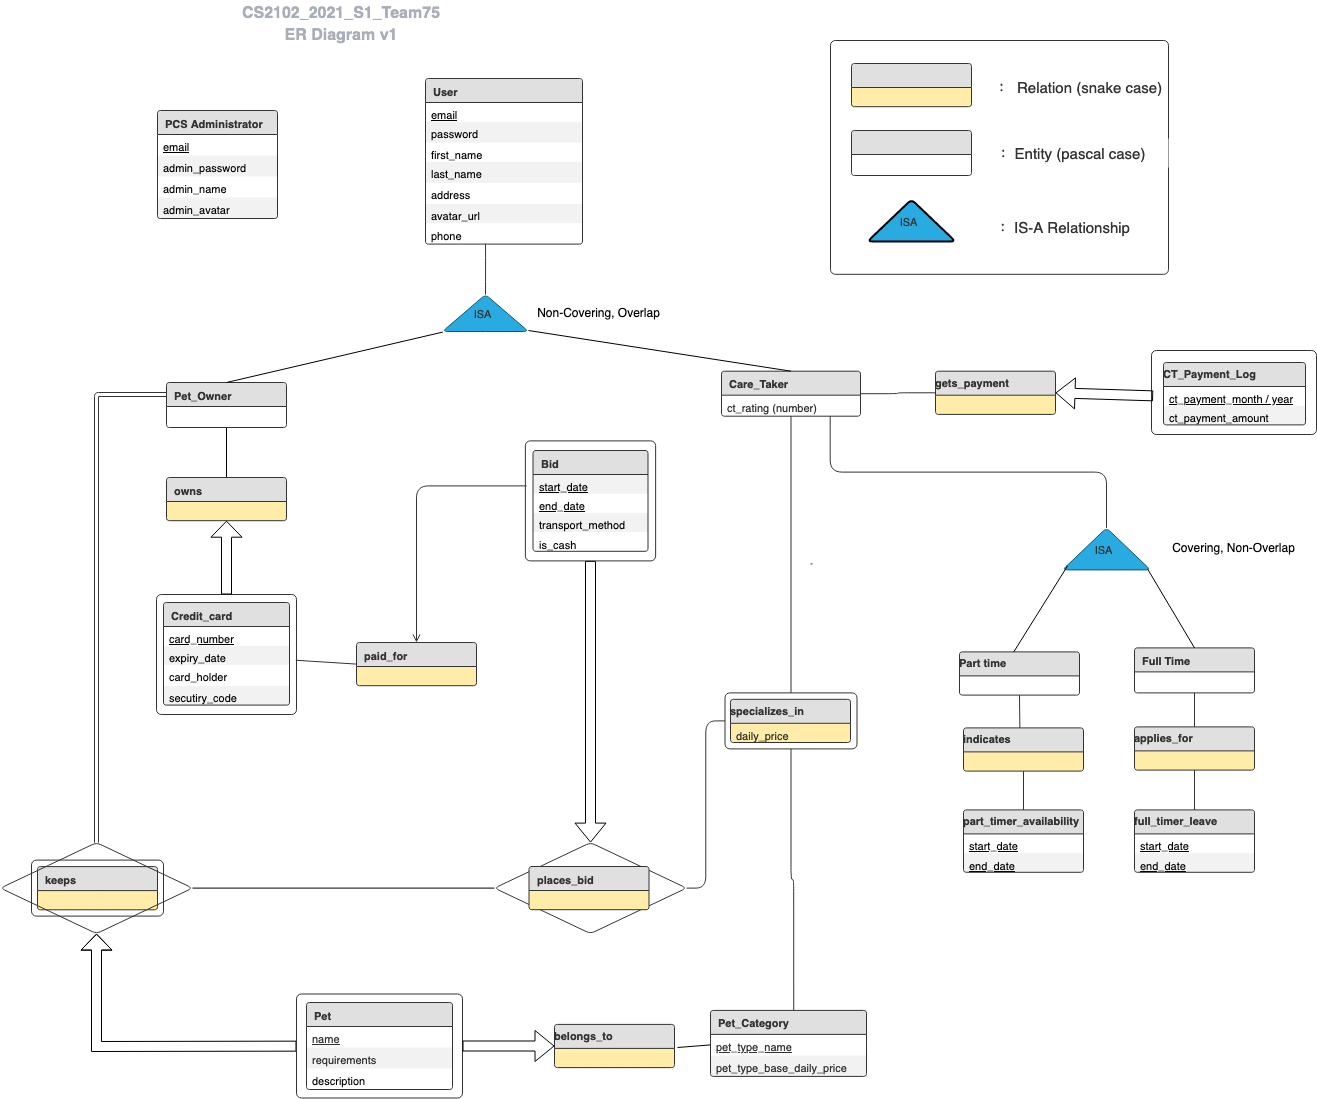
\includegraphics[width=0.95\textwidth,height=\textheight]{./er_diagram.png}
\caption{ER Diagram}
\end{figure}

\hypertarget{relational-schema}{%
\section{Relational Schema}\label{relational-schema}}

\begin{lstlisting}[language=SQL]
CREATE TABLE person(
   email varchar(64) PRIMARY KEY,
   fullname varchar(64) NOT NULL,
   password varchar(64) NOT NULL,
   address varchar(64) NOT NULL,
   phone int NOT NULL,
   role user_role NOT NULL,
   avatar_link varchar
);
\end{lstlisting}

\begin{longtable}[]{@{}ll@{}}
\toprule
\begin{minipage}[b]{0.15\columnwidth}\raggedright
\#\strut
\end{minipage} & \begin{minipage}[b]{0.79\columnwidth}\raggedright
Value\strut
\end{minipage}\tabularnewline
\midrule
\endhead
\begin{minipage}[t]{0.15\columnwidth}\raggedright
FDs\strut
\end{minipage} & \begin{minipage}[t]{0.79\columnwidth}\raggedright
\{email \(\rightarrow\) fullname, password, address, phone, role,
avatar\_link\}\strut
\end{minipage}\tabularnewline
\begin{minipage}[t]{0.15\columnwidth}\raggedright
Normal Forms\strut
\end{minipage} & \begin{minipage}[t]{0.79\columnwidth}\raggedright
BCNF, 3NF\strut
\end{minipage}\tabularnewline
\bottomrule
\end{longtable}

\begin{lstlisting}[language=SQL]
CREATE TABLE pet_category(
   type_name varchar(64) PRIMARY KEY,
   base_daily_price int NOT NULL
);
\end{lstlisting}

\begin{longtable}[]{@{}ll@{}}
\toprule
\# & Value\tabularnewline
\midrule
\endhead
FDs & \{type\_name \(\rightarrow\) base\_daily\_price\}\tabularnewline
Normal Forms & BCNF, 3NF\tabularnewline
\bottomrule
\end{longtable}

\begin{lstlisting}[language=SQL]
CREATE TABLE pet(
   name varchar(64),
   owner varchar(64) REFERENCES person(email),
   category varchar(64) REFERENCES pet_category(type_name) ON UPDATE CASCADE,
   requirements text,
   description text,
   CONSTRAINT pet_id PRIMARY KEY (name, owner)
);
\end{lstlisting}

\begin{longtable}[]{@{}ll@{}}
\toprule
\# & Value\tabularnewline
\midrule
\endhead
FDs & \{name, owner \(\rightarrow\) category, requirements,
description\}\tabularnewline
Normal Forms & BCNF, 3NF\tabularnewline
\bottomrule
\end{longtable}

\begin{lstlisting}[language=SQL]
CREATE TABLE credit_card(
   card_number bigint,
   cardholder varchar(64) REFERENCES person(email),
   expiry_date Date,
   security_code smallint,
   CONSTRAINT credit_card_id PRIMARY KEY (card_number, cardholder)
);
\end{lstlisting}

\begin{longtable}[]{@{}ll@{}}
\toprule
\# & Value\tabularnewline
\midrule
\endhead
FDs & \{card\_number, cardholder \(\rightarrow\) expiry\_date,
security\_code \}\tabularnewline
Normal Forms & BCNF, 3NF\tabularnewline
\bottomrule
\end{longtable}

\begin{lstlisting}[language=SQL]
CREATE TABLE part_time_ct (
   email varchar(64) PRIMARY KEY REFERENCES person(email) ON DELETE CASCADE
);
\end{lstlisting}

\begin{longtable}[]{@{}ll@{}}
\toprule
\# & Value\tabularnewline
\midrule
\endhead
FDs & \{ \}\tabularnewline
Normal Forms & BCNF, 3NF\tabularnewline
\bottomrule
\end{longtable}

\begin{lstlisting}[language=SQL]
CREATE TABLE full_time_ct (
   email varchar(64) PRIMARY KEY REFERENCES person(email) ON DELETE CASCADE
);
\end{lstlisting}

\begin{longtable}[]{@{}ll@{}}
\toprule
\# & Value\tabularnewline
\midrule
\endhead
FDs & \{ \}\tabularnewline
Normal Forms & BCNF, 3NF\tabularnewline
\bottomrule
\end{longtable}

\begin{lstlisting}[language=SQL]
CREATE VIEW caretaker (email, caretaker_status, rating) AS (
   SELECT email, 1, 4.1 FROM  part_time_ct
   UNION
   SELECT email, 2, 4.2 FROM full_time_ct
);
\end{lstlisting}

\begin{lstlisting}[language=SQL]
CREATE TABLE pt_specializes_in (
   email varchar(64) REFERENCES part_time_ct(email) ON DELETE CASCADE,
   type_name varchar(64) REFERENCES pet_category(type_name) ON DELETE CASCADE ON UPDATE CASCADE,
   ct_price_daily int NOT NULL,
   CONSTRAINT pt_specializes_in_id PRIMARY KEY (email, type_name)
);
\end{lstlisting}

\begin{longtable}[]{@{}ll@{}}
\toprule
\# & Value\tabularnewline
\midrule
\endhead
FDs & \{ email, type\_name \(\rightarrow\)
ct\_price\_daily\}\tabularnewline
Normal Forms & BCNF, 3NF\tabularnewline
\bottomrule
\end{longtable}

\begin{lstlisting}[language=SQL]
CREATE TABLE ft_specializes_in (
   email varchar(64) REFERENCES full_time_ct(email) ON DELETE CASCADE,
   type_name varchar(64) REFERENCES pet_category(type_name) ON DELETE CASCADE ON UPDATE CASCADE,
   ct_price_daily int NOT NULL,
   CONSTRAINT ft_specializes_in_id PRIMARY KEY (email, type_name)
);
\end{lstlisting}

\begin{longtable}[]{@{}ll@{}}
\toprule
\# & Value\tabularnewline
\midrule
\endhead
FDs & \{ email, type\_name \(\rightarrow\) ct\_price\_daily
\}\tabularnewline
Normal Forms & BCNF, 3NF\tabularnewline
\bottomrule
\end{longtable}

\begin{lstlisting}[language=SQL]
CREATE VIEW specializes_in (email, type_name, ct_price_daily) as (
   SELECT email, type_name, ct_price_daily FROM pt_specializes_in
   UNION
   SELECT email, type_name, ct_price_daily FROM ft_specializes_in
);
\end{lstlisting}

\begin{lstlisting}[language=SQL]
CREATE TABLE pt_free_schedule (
   email varchar(64) REFERENCES part_time_ct(email) ON DELETE CASCADE,
   start_date date NOT NULL,
   end_date date NOT NULL,
    CONSTRAINT pt_schedule_id PRIMARY KEY (email, start_date, end_date),
   CONSTRAINT end_after_start CHECK (end_date >= start_date),
   CONSTRAINT within_next_year CHECK (extract(year FROM end_date) <= (1 + extract(year FROM CURRENT_DATE)))
);
\end{lstlisting}

\begin{longtable}[]{@{}ll@{}}
\toprule
\# & Value\tabularnewline
\midrule
\endhead
FDs & \{ \}\tabularnewline
Normal Forms & BCNF, 3NF\tabularnewline
\bottomrule
\end{longtable}

\begin{lstlisting}[language=SQL]
CREATE TABLE ft_leave_schedule (
   email varchar(64) REFERENCES full_time_ct(email) ON DELETE CASCADE,
   start_date date NOT NULL,
   end_date date NOT NULL,
   CONSTRAINT ft_schedule_id PRIMARY KEY (email, start_date, end_date),
   CONSTRAINT end_after_start CHECK (end_date >= start_date)
   CONSTRAINT within_next_year CHECK (extract(year FROM end_date) <= (1 + extract(year FROM CURRENT_DATE)))
);
\end{lstlisting}

\begin{longtable}[]{@{}ll@{}}
\toprule
\# & Value\tabularnewline
\midrule
\endhead
FDs & \{ \}\tabularnewline
Normal Forms & BCNF, 3NF\tabularnewline
\bottomrule
\end{longtable}

\begin{lstlisting}[language=SQL]
CREATE TABLE bid (
   ct_email varchar(64) REFERENCES person(email),
   ct_price int NOT NULL,
   start_date DATE NOT NULL,
   end_date DATE NOT NULL,
   is_cash boolean NOT NULL,
   credit_card bigint,
   transport_method transport_method NOT NULL,
   pet_owner varchar(64),
   pet_name varchar(64),
   bid_status bid_status NOT NULL,
   feedback text DEFAULT NULL,
   rating int DEFAULT NULL,
   FOREIGN KEY (pet_owner, credit_card) REFERENCES credit_card(cardholder, card_number),
   FOREIGN KEY (pet_owner, pet_name) REFERENCES pet(owner, name),
   CONSTRAINT bid_id PRIMARY KEY (ct_email, pet_name, pet_owner, start_date, end_date),
   CONSTRAINT valid_date CHECK(end_date >= start_date),
   CONSTRAINT xor_cash_credit CHECK ((is_cash AND credit_card IS NULL) OR (NOT is_cash AND credit_card IS NOT NULL))
);
\end{lstlisting}

\begin{longtable}[]{@{}ll@{}}
\toprule
\begin{minipage}[b]{0.08\columnwidth}\raggedright
\#\strut
\end{minipage} & \begin{minipage}[b]{0.86\columnwidth}\raggedright
Value\strut
\end{minipage}\tabularnewline
\midrule
\endhead
\begin{minipage}[t]{0.08\columnwidth}\raggedright
FDs\strut
\end{minipage} & \begin{minipage}[t]{0.86\columnwidth}\raggedright
\{ ct\_email, pet\_name, pet\_owner, start\_date, end\_date
\(\rightarrow\) ct\_price,is\_cash, credit\_card, transport\_method,
bid\_status, feedback, rating \}\strut
\end{minipage}\tabularnewline
\begin{minipage}[t]{0.08\columnwidth}\raggedright
Normal Forms\strut
\end{minipage} & \begin{minipage}[t]{0.86\columnwidth}\raggedright
BCNF, 3NF\strut
\end{minipage}\tabularnewline
\bottomrule
\end{longtable}

All of our SQL tables are in BCNF, and consequently, 3NF. This is
because all the attributes on the LHS of our functional dependencies are
superkeys of the table.

\hypertarget{application-constraints}{%
\section{Application Constraints}\label{application-constraints}}

\begin{enumerate}
\def\labelenumi{\arabic{enumi}.}
\tightlist
\item
  Users must have a valid-looking email address
\item
  Users register as a Pet Owner or Care Taker after logging in.
\item
  Can only care for pets they specialize in
\item
  Owners and Care
\item
  Both the Pet Owner and Care Taker should agree on how to transfer the
  Pet, which can only be one of the following three:
\item
  Pet Owner deliver
\item
  Care Taker pick up
\item
  Transfer through the physical building of PCS administrator
\item
  Transaction can only be cash or credit card
\item
  A Bid can only progress through status via one of the following
  routes:
\item
  Full Timers
\item
  \passthrough{\lstinline!confirmed!} \(\rightarrow\)
  \passthrough{\lstinline!reviewed!}
\item
  Part Timers
\item
  \passthrough{\lstinline!submitted!} \(\rightarrow\)
  \passthrough{\lstinline!confirmed!}
  \(\rightarrow\)\passthrough{\lstinline!reviewed!}
\item
  \passthrough{\lstinline!submitted!} \(\rightarrow\)
  \passthrough{\lstinline!closed!}
\item
  A Full-time Care Taker will receive a salary of \$3000 per month for
  the first 60 pet-days (number of pets taken care of for how many
  days). They will receive 80\% of their price from any excess pet-day
  as a bonus on top of the \$3000.
\item
  A Part-time Care Taker will take only 75\% of their price as payment.
\end{enumerate}

\hypertarget{interesting-queries}{%
\section{Interesting Queries}\label{interesting-queries}}

\hypertarget{calculating-the-monthly-salary-of-part-timers}{%
\subsection{Calculating the monthly salary of Part
Timers}\label{calculating-the-monthly-salary-of-part-timers}}

\begin{lstlisting}[language=SQL]
SELECT
   sum( (least(ct_bid.end_date, endmonth) + 1 - greatest(ct_bid.start_date, startmonth)) * ct_price) * 0.75 as full_pay,
   to_char(startmonth, 'YYYY-MM') as month_year
   FROM (
      SELECT generate_series(
            date_trunc('month', startend.sd),
            startend.ed, '1 month'
      )::date AS startmonth,
      (generate_series(
            date_trunc('month', startend.sd),
            startend.ed, '1 month'
      ) + interval '1 month' - interval '1 day' )::date AS endmonth
      FROM
            (SELECT min(start_date) AS sd, max(end_date) as ed
            FROM bid
            WHERE ct_email=$1 AND bid_status='confirmed') AS startend
            ORDER BY sd
   ) AS monthly, (SELECT * FROM bid WHERE bid.ct_email=$1 AND bid.bid_status='confirmed') as ct_bid
   WHERE ct_bid.start_date <= monthly.endmonth
   AND monthly.startmonth <= ct_bid.end_date
   AND ct_bid.start_date <= CURRENT_DATE
   GROUP BY monthly.endmonth, monthly.startmonth
   HAVING monthly.endmonth <= CURRENT_DATE
\end{lstlisting}

\begin{itemize}
\tightlist
\item
  Parameters: \$1 here refers to a Part Time Care Takers email
\item
  The challenge here was that the bids were stored as time periods for
  space reasons and this means that the bids could have crossed a month
\item
  We've thus taken the initiative of splitting those periods according
  to month
\item
  Monthly here contains columns startmonth and endmonth which are the
  starting and ending dates respectively for each month
\item
  The cartesian product would then contain multiple entries of a month
  with all possible bids belong to a part timer
\item
  We then proceed to split the bid with least end date and greatest with
  start date to get the days that are only within the month
\end{itemize}

\hypertarget{searching-for-valid-care-takers-based-on-schedule-and-category}{%
\subsection{Searching for valid Care Takers based on schedule and
category}\label{searching-for-valid-care-takers-based-on-schedule-and-category}}

\begin{lstlisting}[language=SQL]
SELECT fullname, phone, address, email, avatar_link as avatarUrl, caretaker_status as caretakerStatus, rating, ct_price_daily as ctPriceDaily, type_name as typeName FROM (
   SELECT email, $3 as type_name FROM
      (SELECT DISTINCT email
            FROM pt_free_schedule
            WHERE start_date <= $1 AND end_date >= $2
      UNION
      SELECT email FROM full_time_ct ftct
            WHERE NOT EXISTS (
               SELECT 1 FROM ft_leave_schedule fts
               WHERE fts.email = ftct.email
               AND start_date <= $1
               AND end_date >= $2
            )
      ) as free_sched
      WHERE EXISTS (
            SELECT 1 FROM specializes_in s WHERE type_name = $3 AND s.email=free_sched.email
      )
   ) as s NATURAL JOIN person NATURAL JOIN caretaker NATURAL JOIN specializes_in
\end{lstlisting}

\begin{itemize}
\tightlist
\item
  Parameters: \$1: start date of request, \$2: end date of request, \$3
  category of pet requested
\item
  This query first looks for available Care Takers

  \begin{itemize}
  \tightlist
  \item
    It does so by checking that the start date of the potential bid is
    within any period of any Part Timers free schedule and that it is
    not within any period of any Full Timers leave schedule
  \end{itemize}
\item
  Then it checks that those Care Takers do specialize in that pet
  category via \passthrough{\lstinline!type\_name!}
\end{itemize}

\hypertarget{calculating-full-time-pay}{%
\subsection{Calculating Full Time Pay}\label{calculating-full-time-pay}}

\begin{lstlisting}[language=SQL]
SELECT COALESCE(d4.fullpay, 3000.0) AS full_pay,
        COALESCE(d4.bonus, 0) AS bonus,
        d3.month AS month_year FROM
            (SELECT SUM(ct_price)*0.8+3000 AS fullpay,
                    SUM(ct_price)*0.8 AS bonus,
                    concat(yy, '-', mm) AS month FROM
                (SELECT ct_price, dd, mm, yy,
                        ROW_NUMBER() OVER (PARTITION BY mm, yy
                        ORDER BY concat(date, ct_price, pet_owner, pet_name, ct_email) ASC) AS r FROM
                    (SELECT pet_owner, pet_name, ct_email, ct_price,
                            to_char(gen_dates.date,'DD') AS dd,
                            to_char(gen_dates.date,'MM') AS mm,
                            to_char(gen_dates.date, 'YYYY') AS yy,
                            date FROM
                        (SELECT generate_series(
                                    date_trunc('month', startend.sd),
                                    startend.ed, '1 day'
                                )::date AS date FROM
                            (SELECT min(start_date) AS sd, CURRENT_DATE as ed FROM
                                bid
                                WHERE ct_email=$1
                            ) AS startend ORDER BY sd
                        ) AS gen_dates, (SELECT * FROM bid WHERE ct_email=$1) AS p
                        WHERE gen_dates.date >= p.start_date AND gen_dates.date <= p.end_date
                        ORDER BY gen_dates.date
                    ) AS monthdates
                ) rank_price WHERE r > 60 GROUP BY mm, yy
            ) AS d4
            RIGHT JOIN
            (SELECT
                    to_char(generate_series(
                        date_trunc('month', startend.sd),
                        startend.ed, '1 month'
                    )::date, 'YYYY-MM') AS month FROM
                (SELECT min(start_date) AS sd, CURRENT_DATE AS ed FROM bid
                    WHERE ct_email=$1
                ) AS startend
            ) AS d3
            ON d4.month=d3.month
        WHERE (Date(d3.month||'-01') + '1 month'::interval - '1 day'::interval) <= CURRENT_DATE
\end{lstlisting}

\begin{itemize}
\tightlist
\item
  Parameters: \$1: Full Time CareTaker email
\item
  This query is sort of an expansion of generating a part timer's salary
  but is far more complex with the need to find the first 60 pet days
\item
  The high overview is to first generate the bonus, d3, from the 61st
  pet day onwards and right outer join (d4 on the right) it with a
  table, d4, that captures all the months since the Full Timer has begun
  work, then doing a coalesce for months in the d4 that don't have any
  value in d3
\item
  To get the bonus: generate a date for every month where a bid exists
  and do a cartesian product with bid and select dates that exist in any
  bid period
\item
  we then did a partition by month, year as well as generated an
  enumeration over each partition with
  (\passthrough{\lstinline!ROW\_NUMBER!}) so that we could get the first
  60 pet days

  \begin{itemize}
  \tightlist
  \item
    We've also done it such that we've ordered each partition by date
    first then \passthrough{\lstinline!ct\_price!} (Care Taker Price) in
    ascending order within each (\passthrough{\lstinline!month!},
    \passthrough{\lstinline!year!})
  \item
    So we hope to have very happy Full Timers who get the better rates
    beyond the first 60 pet days
  \end{itemize}
\item
  Next is the right outer join with d4, which gives us some entries in
  d3 that are NULL which represent months which the Full Timer has not
  had any bids requested

  \begin{itemize}
  \tightlist
  \item
    We solve this by Coalescing these NULL values with a standard 3000
    salary and bonus of 0
  \end{itemize}
\end{itemize}

\hypertarget{interesting-triggers}{%
\section{Interesting Triggers}\label{interesting-triggers}}

\hypertarget{pet-limit-for-care-takers}{%
\subsection{Pet Limit for Care Takers}\label{pet-limit-for-care-takers}}

\begin{lstlisting}[language=SQL]
CREATE OR REPLACE FUNCTION pet_limit()
RETURNS TRIGGER AS
$t$
DECLARE pet_count INTEGER;
DECLARE transgression INTEGER;

BEGIN
    select
        case
            when caretaker_status=2 OR rating > 4 then 4
            else 1 end
        into pet_count from caretaker where email=NEW.ct_email;

    select count(*) into transgression FROM
        (select
            dates.date
            from (
                select
                    generate_series(
                        date_trunc('month', NEW.start_date),
                        NEW.end_date, '1 day'
                    )::date as date
            ) as dates, (select * FROM bid WHERE ct_email=NEW.ct_email) as p
            where dates.date >= p.start_date and dates.date <= p.end_date
        ORDER BY dates.date) as overlapDates
    group by overlapDates.date
    having count(*) > pet_count;

    insert into count_limit values (transgression);

    IF transgression > 0 THEN
        RAISE EXCEPTION 'limit reached for period!';
    ELSE
        RETURN NEW;
    END IF;
END;
$t$ LANGUAGE PLpgSQL;

CREATE TRIGGER check_pet_limit
BEFORE INSERT ON bid
FOR EACH ROW EXECUTE PROCEDURE pet_limit();
\end{lstlisting}

\begin{itemize}
\tightlist
\item
  pet\_count is the limit on the number of pets a Care Taker can care
  for on any day.

  \begin{itemize}
  \tightlist
  \item
    it has been configured based on Part Time/Full Time and rating
  \item
    the actual limit is pet\_count + 1 since this trigger is done before
    insertion
  \end{itemize}
\item
  Transgressions is the count of the days when a Care Taker has more
  than \passthrough{\lstinline!pet\_count!} number of pets on any day
\item
  We do this check by generating dates from start to end of the new bid
  for every bid that overlaps the new bid and then checking that the
  count for each date does not exceed the
  \passthrough{\lstinline!pet\_count!}
\end{itemize}

\hypertarget{two-consecutive-150-working-days-constraint}{%
\subsection{Two consecutive 150 working days
Constraint}\label{two-consecutive-150-working-days-constraint}}

\begin{lstlisting}[language=SQL]
CREATE OR REPLACE FUNCTION ft_150_constraint()
RETURNS TRIGGER AS
$t$
DECLARE
    count_150 NUMERIC;
    count_300 NUMERIC;
    new_end_year NUMERIC;
    new_start_year NUMERIC;
BEGIN

    SELECT extract(year from NEW.start_date) into new_start_year;
    SELECT extract(year from NEW.end_date) into new_end_year;

    select COUNT(*) into count_150 FROM (
        select * from (
            select *, row_number() over (partition by 1) as r1 from (
                select (Date(new_start_year||'-01-01')-'1 day'::interval) as ed1
                union
                SELECT end_date as ed1 FROM ft_leave_schedule f1
                WHERE email=NEW.email AND start_date >= Date(new_start_year||'-01-01') order by ed1 ASC
            ) t1
        ) ord1 inner join
        (
            select *, row_number() over (partition by 1) as r2 from (
                select (Date(new_end_year||'-01-01')+'1 year'::interval) as sd2
                union
                select start_date as sd2 FROM ft_leave_schedule f2
                WHERE email=NEW.email AND start_date >= Date(new_start_year||'-01-01') order by sd2 ASC
            ) t2
        ) ord2 on ord1.r1=ord2.r2
    ) as cc
    WHERE Date(cc.sd2)-Date(cc.ed1) > 150;

    select COUNT(*) into count_300 FROM (
        select * from (
            select *, row_number() over (partition by 1) as r1 from (
                select (Date(new_start_year||'-01-01')-'1 day'::interval) as ed1
                union
                SELECT end_date as ed1 FROM ft_leave_schedule f1
                WHERE email=NEW.email AND start_date >= Date(new_start_year||'-01-01') order by ed1 ASC
            ) t1
        ) ord1 inner join
        (
            select *, row_number() over (partition by 1) as r2 from (
                select (Date(new_end_year||'-01-01')+'1 year'::interval) as sd2
                union
                select start_date as sd2 FROM ft_leave_schedule f2
                WHERE email=NEW.email AND start_date >= Date(new_start_year||'-01-01') order by sd2 ASC
            ) t2
        ) ord2 on ord1.r1=ord2.r2
    ) as cc
    WHERE Date(cc.sd2)-Date(cc.ed1) > 300;

    IF new_start_year != new_end_year THEN
        IF count_300 = 2 OR count_150 = 4 OR (count_150 = 2 AND count_300 = 1) THEN
            RETURN NEW;
        ELSE
            RAISE EXCEPTION 'No 2 times 150 consecutive working days!';
        END IF;
    ELSE
        IF count_150 = 2 OR count_300 = 1 THEN
            RETURN NEW;
        ELSE
            RAISE EXCEPTION 'No 2 times 150 consecutive working days!';
        END IF;
    END IF;

END;
$t$ LANGUAGE PLpgSQL;
CREATE TRIGGER check_ft_150
AFTER INSERT ON ft_leave_schedule
FOR EACH ROW EXECUTE PROCEDURE ft_150_constraint();
\end{lstlisting}

\begin{itemize}
\tightlist
\item
  This query works by first getting the start and end years of the start
  and end dates of the new leave schedule
\item
  The first and second queries are identical except that one checks for
  150 day gaps and the second checks for 300 day gaps
\item
  Overview: We want to check the gaps between each leave schedule to see
  if it is either a 150 day gap or a 300 day gap
\item
  So what we have done is to prepend the start of the year to t1 and
  append the end of the year to t2
\item
  t1 contains the end dates of each leave schedule as well as the start
  date of the year
\item
  t2 contains the start dates of each leave schedule as well as the end
  date of the year
\item
  We then order both tables by ascending order of the end dates and
  start dates respectively for t1 and t2
\item
  Next we use row number again to generate an enumeration and join the
  tables so that we get the end dates and start dates in the same row
  such that start date - end date gives us the gap between each leave
  schedule
\item
  We then check the count of the 150/300 day gaps
\item
  At the end, it's a conditional based on whether the leave is applied
  across 2 years or is in a single year
\end{itemize}

\hypertarget{part-time-availability-overlap-check}{%
\subsection{Part time availability overlap
check}\label{part-time-availability-overlap-check}}

\begin{lstlisting}[language=SQL]
CREATE OR REPLACE FUNCTION no_bid_overlap()
RETURNS TRIGGER AS
$t$
DECLARE overlap INTEGER;
DECLARE pt_overlap INTEGER;
BEGIN
    -- only allow for multiple submitted bids with overlap and essentially are the same bid
    SELECT COUNT(*) INTO overlap FROM bid
        WHERE NEW.start_date <= end_date
        AND NEW.end_date >= start_date
        AND NEW.pet_owner=pet_owner
        AND NEW.pet_name=pet_name;

    SELECT COUNT(*) INTO pt_overlap FROM bid b
        WHERE NEW.start_date=b.start_date
        AND NEW.end_date=b.end_date
        AND NEW.pet_owner=b.pet_owner
        AND NEW.pet_name=b.pet_name
        AND b.bid_status='submitted';

    IF (overlap-pt_overlap) > 0 THEN
        RAISE EXCEPTION 'Bid for pet overlaps!';
    ELSE
        RETURN NEW;
    END IF;
    RETURN NEW;
END;
$t$ LANGUAGE PLpgSQL;

CREATE TRIGGER check_no_bid_overlap
BEFORE INSERT ON bid
FOR EACH ROW EXECUTE PROCEDURE no_bid_overlap();
\end{lstlisting}

\begin{itemize}
\tightlist
\item
  This trigger serves to enforce no overlapping bids
\item
  A bid overlaps is if it's for the same pet and the dates overlap
  irregardless of Care Taker bided for
\item
  This is with the caveat that there can be multiple identical bids only
  if all the bids are for Part Time Care Takers
\item
  A bid is identical if it is for the same pet with the same start and
  end dates. But identical bids can be placed on different Care Takers
\item
  This is due to our option for Part Timers to accept or reject bids
\item
  We enforced this by counting the number of overlaps and then
  subtracting off the overlaps resulting from identical bids on Part
  Timers
\item
  This count should thus be 0
\end{itemize}

\hypertarget{technical-specifications}{%
\section{Technical Specifications}\label{technical-specifications}}

Our application is implemented with an Express/Node backend that serves
a ReactJS frontend. Subsequently the frontend client communicates with
the Node backend using RESTful API calls.

Our application is deployed on Heroku with Docker. PR preview is powered
by Heroku Review Apps.

\begin{itemize}
\tightlist
\item
  Frontend:

  \begin{itemize}
  \tightlist
  \item
    React v16.5
  \item
    Ant Design v4.5
  \item
    Typescript
  \item
    Axios
  \end{itemize}
\item
  Backend:

  \begin{itemize}
  \tightlist
  \item
    Typescript
  \item
    Express
  \item
    Node
  \item
    \passthrough{\lstinline!passport-jwt!}
  \end{itemize}
\item
  Database: PostgreSQL 12.1
\end{itemize}

\hypertarget{screenshots}{%
\section{Screenshots}\label{screenshots}}

\begin{figure}
\centering
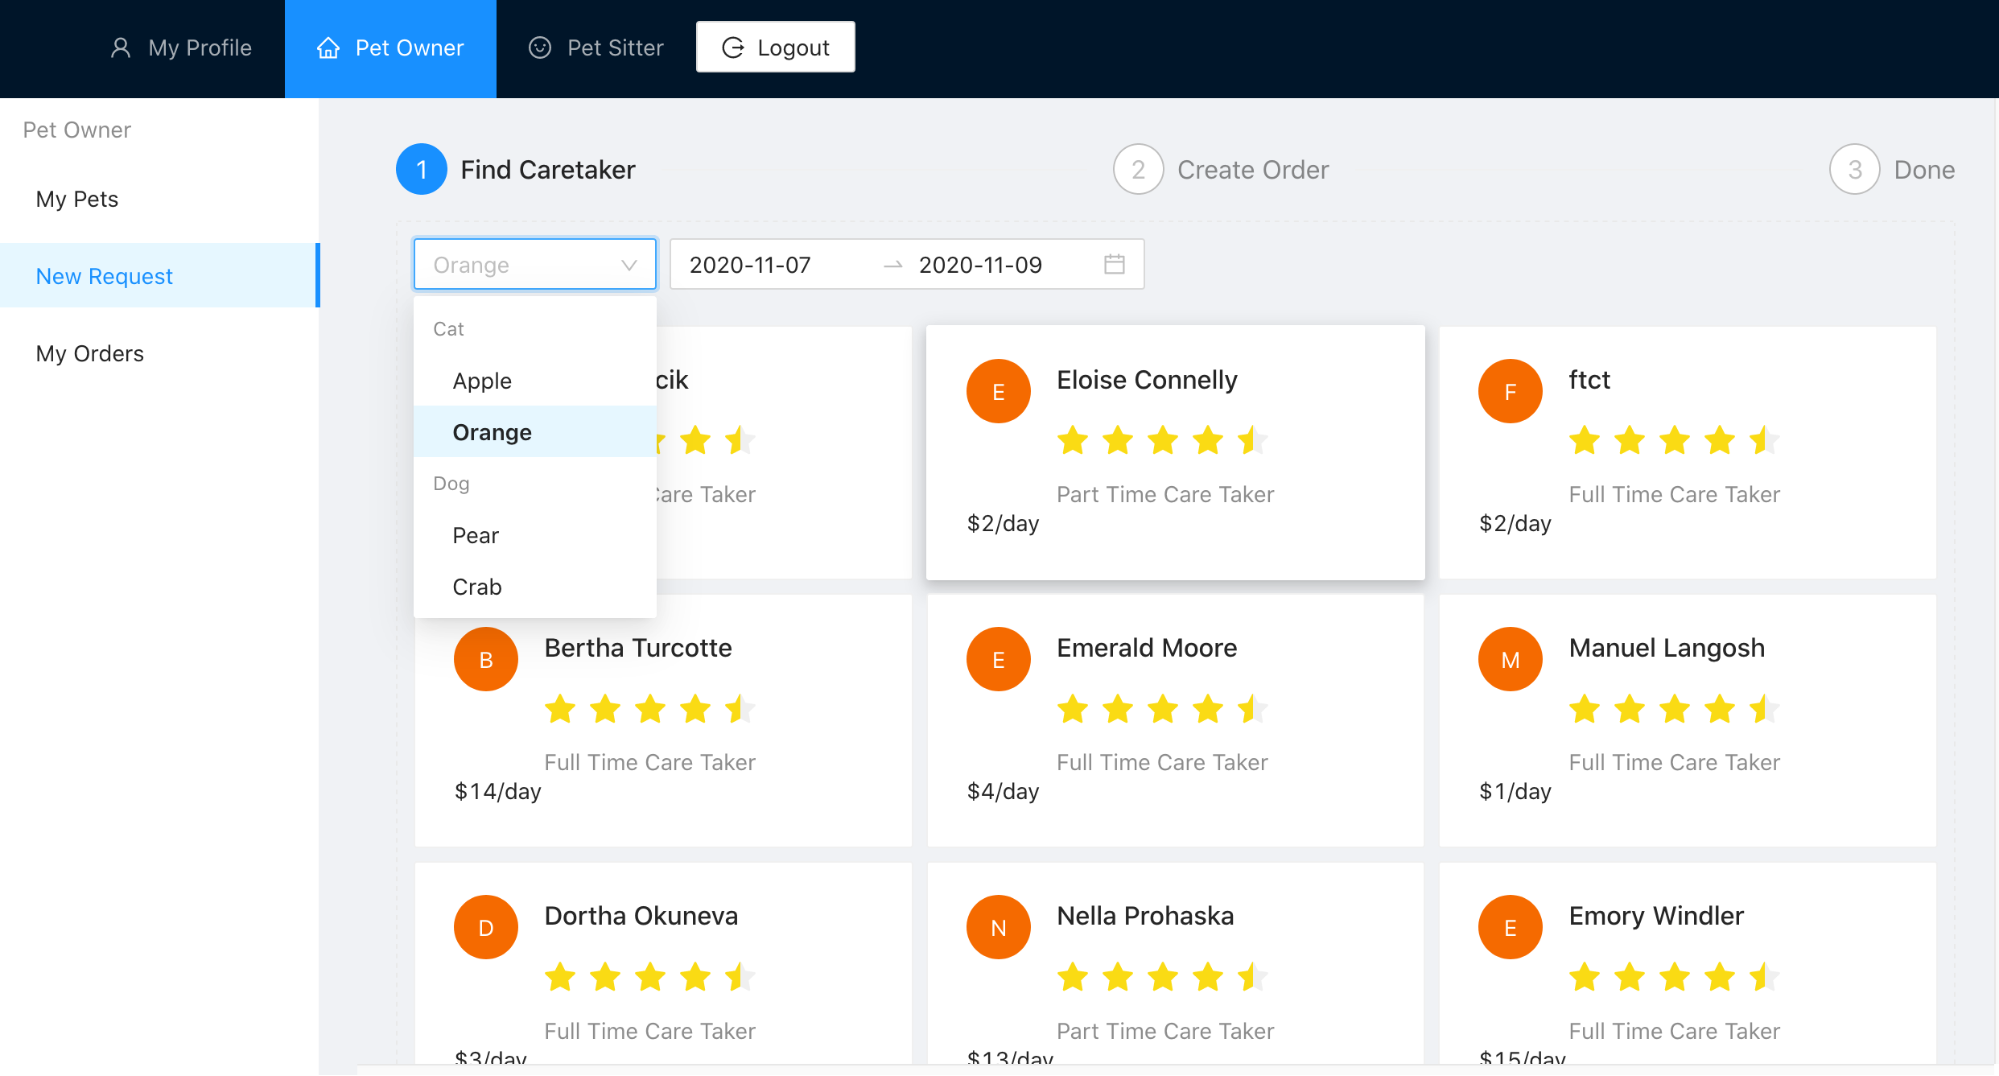
\includegraphics{find-caretaker.png}
\caption{Finding Caretaker}
\end{figure}

Finding Caretaker:

\begin{enumerate}
\def\labelenumi{\arabic{enumi}.}
\tightlist
\item
  Choose the Pet in the top-left box;

  \begin{enumerate}
  \def\labelenumii{\arabic{enumii}.}
  \tightlist
  \item
    the Pets are collected into their respective categories
  \end{enumerate}
\item
  Choose the intended Start and End date
\item
  Browse the list of Caretakers and their information; click the card to
  proceed to the next step
\end{enumerate}

\begin{figure}
\centering
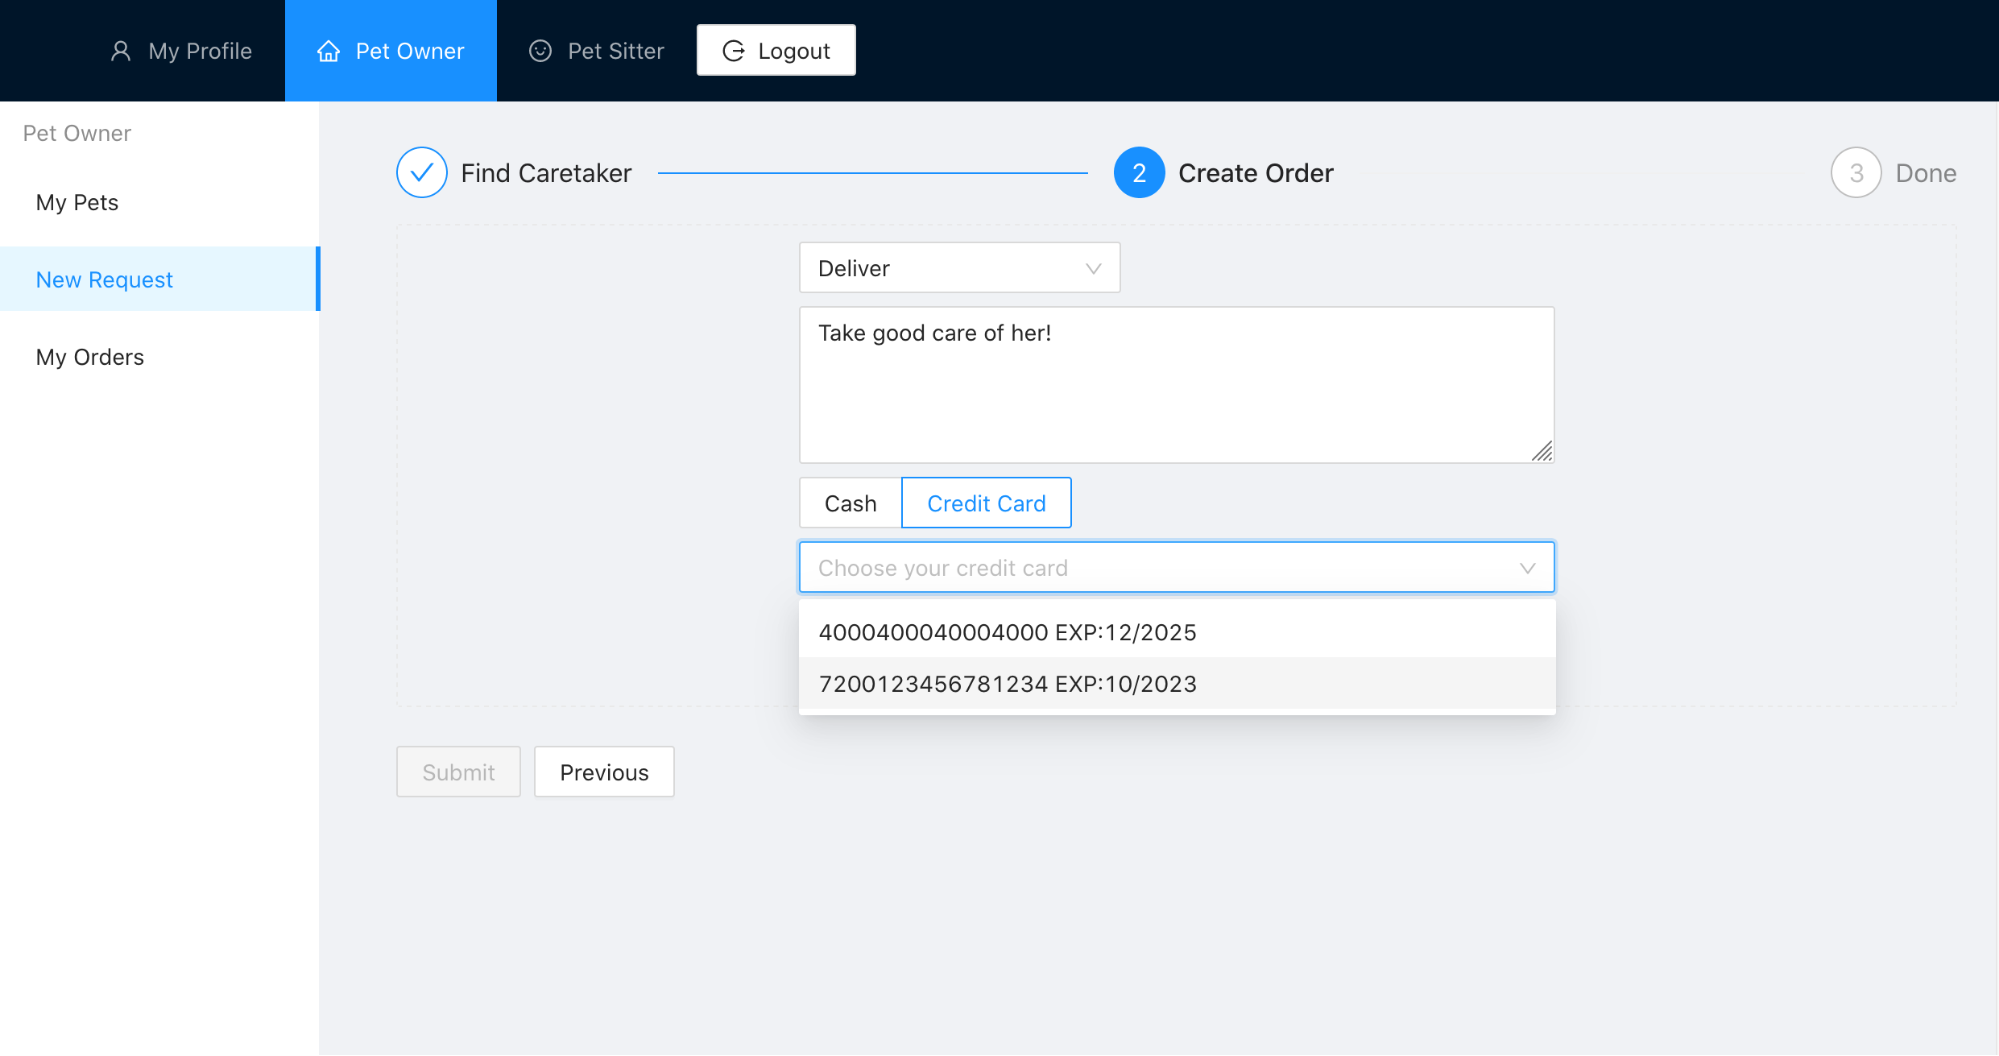
\includegraphics{create-order.png}
\caption{Creating a New Request}
\end{figure}

Creating Order:

\begin{enumerate}
\def\labelenumi{\arabic{enumi}.}
\tightlist
\item
  Choose the delivery methods among Deliver, Pickup and Transit through
  PCS
\item
  Choose either paying by Cash or Credit Card;

  \begin{enumerate}
  \def\labelenumii{\arabic{enumii}.}
  \tightlist
  \item
    The Credit Cards are organized in a drop-down selection box
  \item
    Choose a credit card, if applicable
  \end{enumerate}
\end{enumerate}

\begin{figure}
\centering
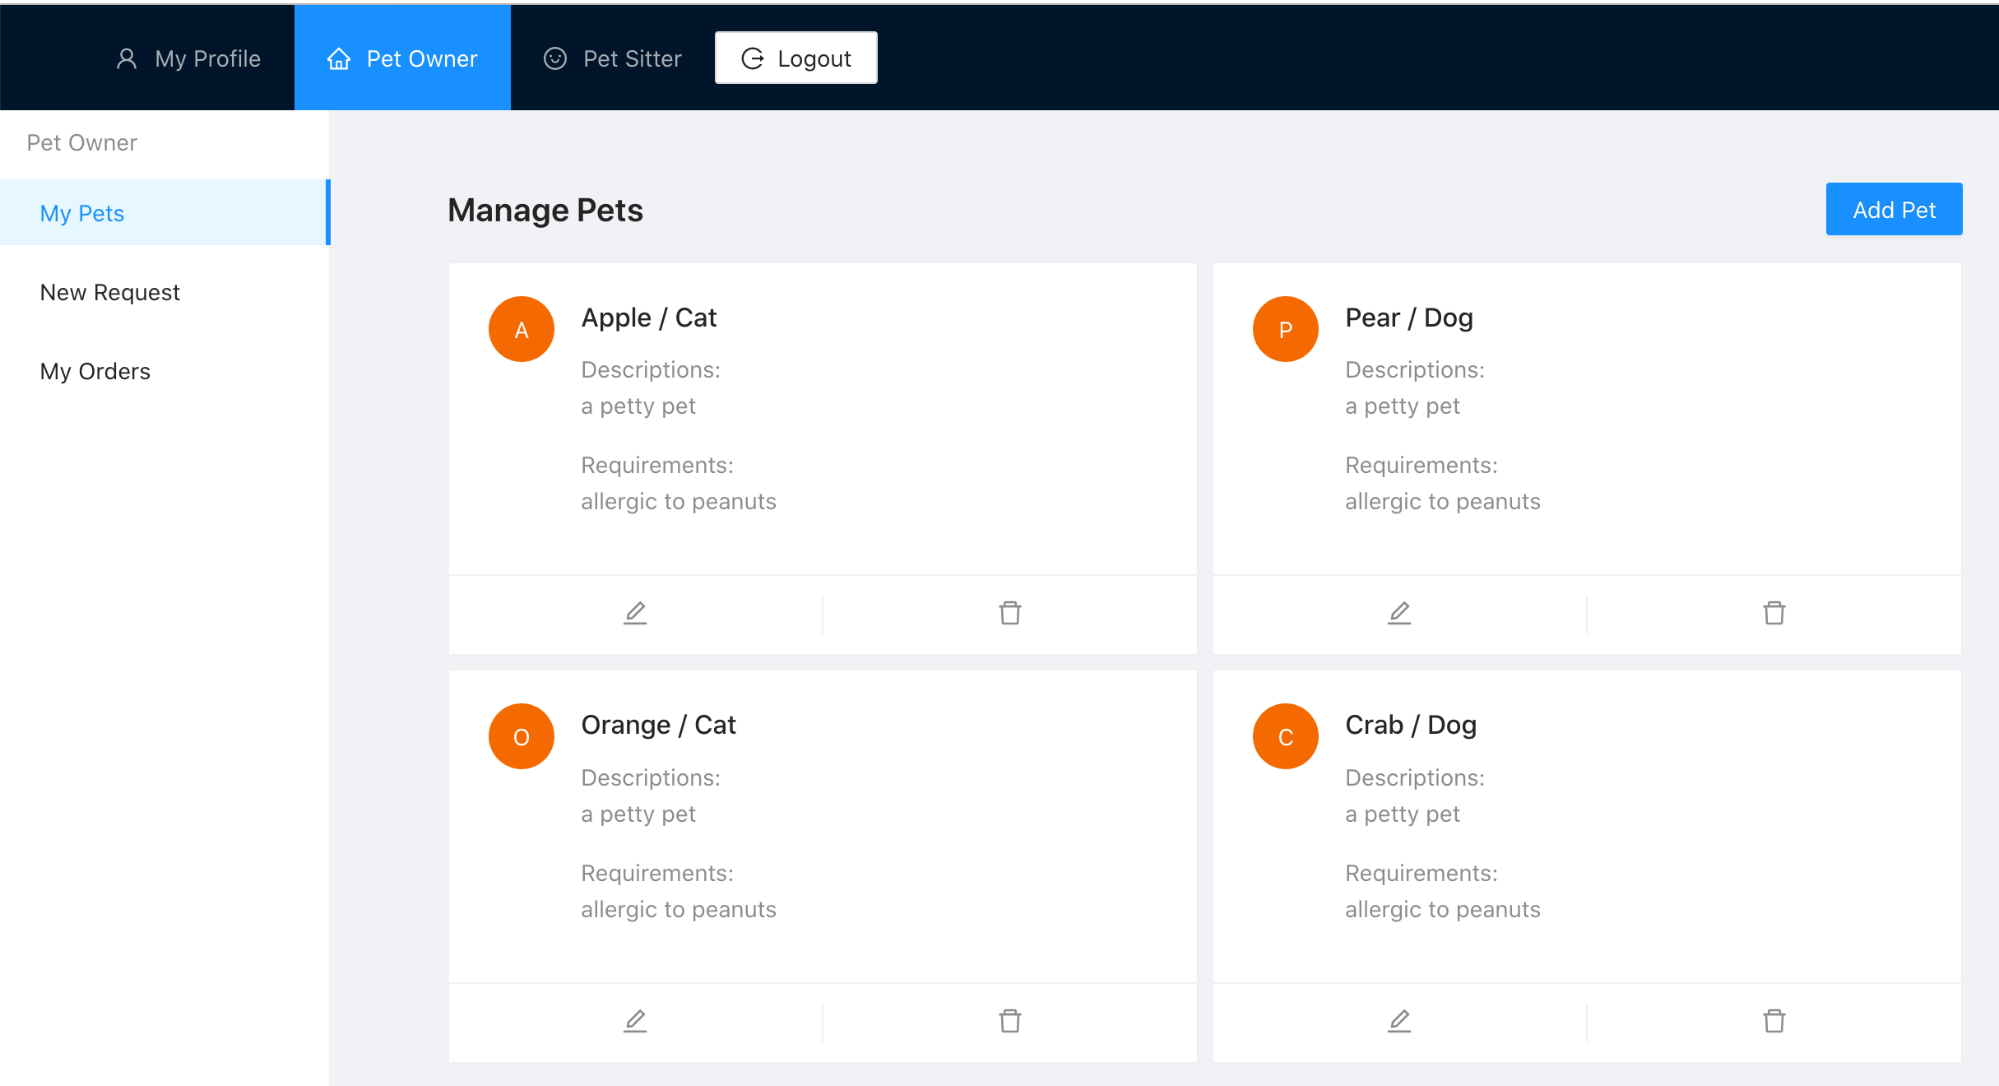
\includegraphics{manage-pet.png}
\caption{Managing Pets}
\end{figure}

\hypertarget{summary}{%
\section{Summary}\label{summary}}

One problem that we faced along the way is the frontend-backend
integration. As \passthrough{\lstinline!pg!} runs on JavaScript, the
properties of the Query Result rows are not known at compile-time. Even
though we adopted TypeScript, we were not able to type-check the
outgoing JSON objects. This causes a lot of trouble, since no warning is
given when the object schema changes. Front-end will encounter error
accessing undefined object keys that existed before the schema change.

Another major challenge is the discrepancies between the key names
between the database and backend and frontend. Since postgres is
case-insensitive, we have to be wary of converting the key from
\passthrough{\lstinline!snake\_case!} to
\passthrough{\lstinline!camelCase!} in our code. This becomes confusing
when different team members do not follow the convention, which
sometimes leaks into the frontend, causing an avalanche of runtime
errors. A way to overcome this is to state the conventions followed in
some form of documentations such as Github Wiki beforehand. Timely
communication is also crucial in preventing inconsistency and reducing
integration overhead.

However, we were amazed by the type-safety brought by TypeScript in our
front-end codebase. Without the type guidance, we will not be able to
fix the errors caused by the schema changes quickly.

Some decisions on the application constraints are not fully thought out
during the ER diagram design phase. This has led to repeated changes in
schema and endpoints to cater to new constraints. This could have been
prevented by starting to consider and document the constraints early.

Overall, we felt that the use of the ER diagram has helped us greatly in
communicating database design requirements. Functional dependency
analysis is also easier when the relational schema follows the ER
diagram closely and is concise and clear. We have learnt that modelling
a real world problem can be done more effectively and efficiently with
systematic knowledge on relational schema and functional dependencies.

\end{document}
